\documentclass{homework}
\usepackage{lipsum}
\usepackage{cancel}
\usepackage{amsthm}
\usepackage{cleveref}
\usepackage{upgreek}
\usepackage[framed]{mcode}
\usepackage{mathrsfs}
\usepackage{tikz}
\usepackage{units}
\usetikzlibrary{matrix}
\newtheorem{lemma}{Lemma}
\DeclareMathOperator*{\argmin}{arg\,min}

\title{Kevin Joyce}
\course{Math 514 - Inverse Problems - Homework 7}
\author{Kevin Joyce}
\docdate{\today}
\begin{document} 
\newcommand{\figref}[1]{\figurename~\ref{#1}}
\renewcommand{\bar}{\overline}
\renewcommand{\hat}{\widehat}
\renewcommand{\SS}{\mathcal S}
\newcommand{\HH}{\mathscr H}
\newcommand{\mom}{\widetilde}
\newcommand{\mle}{\widehat \Uptheta}
\newcommand{\eps}{\varepsilon}
\newcommand{\todist}{\stackrel{D}\longrightarrow}
\newcommand{\toprob}{\stackrel{p}\longrightarrow}
\newcommand{\TTheta}{\overline{\underline \Theta} }
\newcommand{\del}{\partial}
\newcommand{\approxsim}{\overset{\cdotp}{\underset{\cdotp}{\sim}}}

\problem{Bardsley 4.6. Let $h=1/n$ and $s_i = (i-1/2)h$ for $i=1,\dots,n$.  Expand $x(s_i+h)$ in a Taylor series about $s_i$ and show that
$$
  x'(s_i) = \frac{x(s_{i+1}) - x(s_i)}{h} + E_s,\quad i=1,\dots,n,
$$
where $E_s$ has order $h$.  Assume that $x$ is sufficiently differentiable.  From this expresssion, derive the forward difference matrices $\vect D$ for each of the zero (an $(n+1)\times n$ matrix), periodic (an $n\times n$ matrix), and Neumann (an $(n-1)\times n$ matrix) boundary conditions assumptions.  Verify that each satisfies $\vect D^T\vect D = \vect L$, where $\vect L$ is discrete negative second derivative with the corresponding boundary condition.
}
\begin{solution}
Assuming that $x$ is sufficiently smooth at each $s_i$ to admit a Taylor series, then
$$
  x(t) = x(s_i) + x'(s_i)(t - s_i) + O\left((t-s_i)^2\right)
$$
and evaluating at $s_{i+1} = s_i+h$,
$$
  x(s_{i+1}) = x(s_i) + x'(s_i)h + O(h^2).
$$
Solving for $x'(s_i)$,
$$
  x'(s_i) = \frac{x(s_{i+1}) - x(s_i)}{h} + O(h).
$$
Let us drop order $h$ terms and denote $x_i = x(s_i)$. Then, if we assume $x_0 = x_{n+1} =
0$ (zero BC) then $[\vect{D x}]_1 = x_1/h$, $[\vect{Dx}]_i = (x_{i+1} -
x_i)/h$ for $1<i\le n$, and $[\vect{Dx}]_{n+1}=-x_n/n$. Hence the matrix is of the form
$$
  \vect D = h^{-1}\begin{bmatrix}
  1      &        &        \\
  -1     & 1      &        \\
         & \ddots & \ddots \\
         &        & -1
  \end{bmatrix}
  \quad\text{and}\quad
  \vect D^2 = h^{-2}\begin{bmatrix}
  2      & -1     &        &    \\
  -1     & 2      & \ddots &    \\
         & \ddots & \ddots & -1 \\
         &        & -1     & 2
  \end{bmatrix}.
$$
If we assume $x_0 = x_n$ (periodic BC), then $[\vect{Dx}]_1 = (x_1 - x_n)/h$,
$[\vect{Dx}]_i = (x_i - x_{i-1})/h$, and $[\vect{Dx}]_n = (x_n - x_1)/h$. The matrix has the form
$$
  \vect D = h^{-1} \begin{bmatrix} 
  1      &        &   -1   \\
  -1     & 1      &        \\
         & \ddots &        \\
         & -1     & 1
  \end{bmatrix}
  \quad\text{ and }\quad
  \vect D^2 = h^{-2}\begin{bmatrix}
  2      & -1     &        & -1 \\
  -1     & 2      & \ddots &    \\
         & \ddots & \ddots & -1 \\
  -1     &        & -1     & 2
  \end{bmatrix}.
$$
For Neumann boundary conditions, we remove the first and last rows of zeros so that
$$
  \vect D = h^{-1} \begin{bmatrix} 
  -1     & 1      &        \\
         & \ddots &        \\
         & -1     & 1
  \end{bmatrix}
  \quad\text{and}\quad
  \vect D^2 = h^{-2}\begin{bmatrix}
  1      & -1     &        &    \\
  -1     & 2      & \ddots &    \\
         & \ddots & \ddots & -1 \\
         &        & -1     & 1
  \end{bmatrix}.
$$
\end{solution}
\newpage

\problem{Bardsley 4.7. Show that if $p(\vect x|\delta) \propto \exp\left(-\frac\delta2 \vect{x}^T\vect{Lx}\right)$, then the MAP solution is also the solution of 
\begin{equation}
\left(\vect A^T\vect A - (\delta/\lambda) \vect L\right)\vect x = \vect A^T \vect b\label{normeq} \tag{4.35}.
\end{equation}  Assume that the nullspace of $\vect A$ and $\vect L$ don't intersect, so that $\vect A^T\vect A + \alpha \vect L$ is invertible.}


\begin{solution}
  By Bayes' theorem, the posterior is proportional to
  $$
  \exp\left( - \frac\lambda2\|\vect{Ax} - \vect b\|^2 - \frac{\delta}{2}\vect x^T\vect{Lx}\right),
  $$
  which is maximized when 
  $$
  \ell(\vect x) = \frac\lambda2\|\vect{Ax} - \vect b\|^2 + \frac{\delta}{2}\vect x^T\vect{Lx}
  $$
  is minimized.  Recall that the gradient of a quadratic form $\vect x^T\vect{Cx}$ is given by $2\vect{Cx}$ (see homework 3). 
  Denoting the inner product between two vectors as $\vect x \cdot \vect y$, we have
  \begin{align*}
    \nabla \ell(\vect x) 
    &= \frac{\lambda}2 \nabla \vect x^T \vect A^T \vect A\vect x - \frac{\lambda}2\nabla 2\vect x \cdot (\vect A^T \vect b) + \frac{\lambda}2\nabla \vect b^T\vect b -\frac{\delta}2 \nabla \vect x^T\vect{Lx}\\
    &= \lambda \vect A^T\vect{Ax} - \lambda \vect A^T \vect b - \delta\vect{Lx} \\
    &= \lambda \Big(\vect A^T \vect A - (\lambda/\delta)\vect{Lx}\Big)\vect x - \lambda \vect A^T\vect b= 0\\
  \end{align*}
  if and only if \eqref{normeq} (with nullspace conditions) holds.
\end{solution}

\problem{Bardsley 4.10. \emph{Kernel Reconstruction:} Modify \texttt{Deblur1dGMRF.m} and \texttt{Debulur1dIGMRF.m} so that they implement the kernel reconstruction problem from Chapters 1 and 2. }

\begin{minipage}{.5\textwidth}
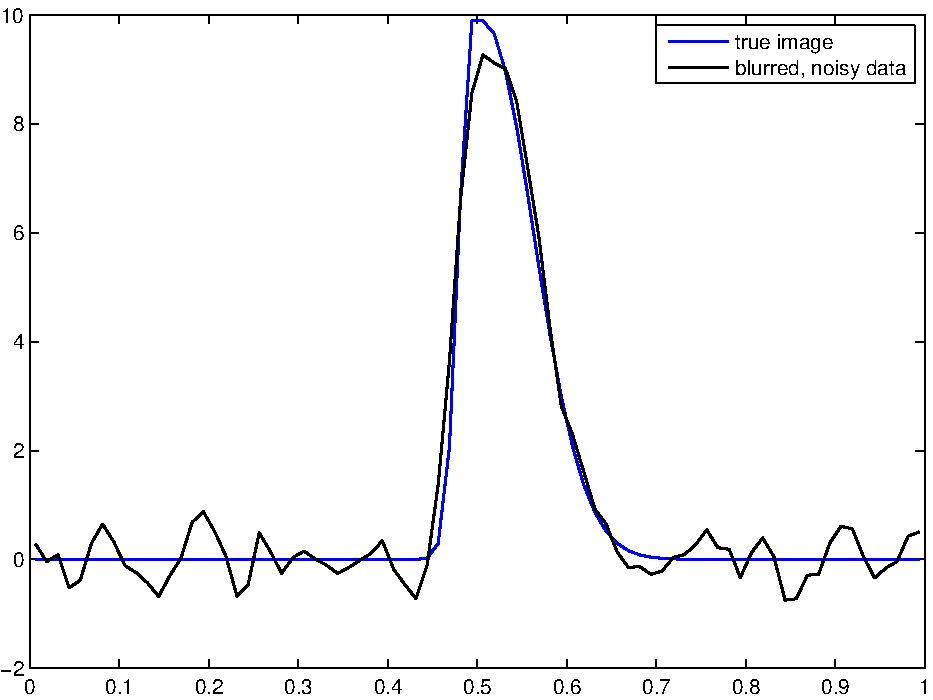
\includegraphics[width=\textwidth]{psfrecon_gmrf.pdf}
\end{minipage}
\begin{minipage}{.5\textwidth}
The MAP estimator with Gaussian priors was implemented in \texttt{PSFrecon1dGMRF.m} modified from \texttt{Deblur1dGMRF}. The resulting regularization is given to the left. Note that the regularization is poor on the tails.
\end{minipage}
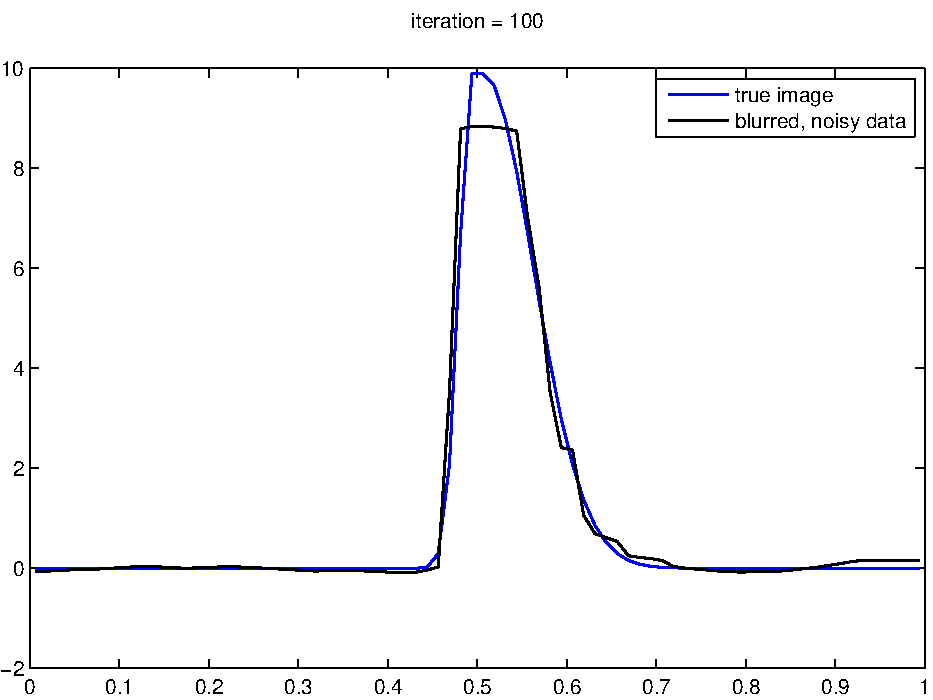
\includegraphics[width=.25\textwidth]{psfrecon_igmrf_01.pdf}
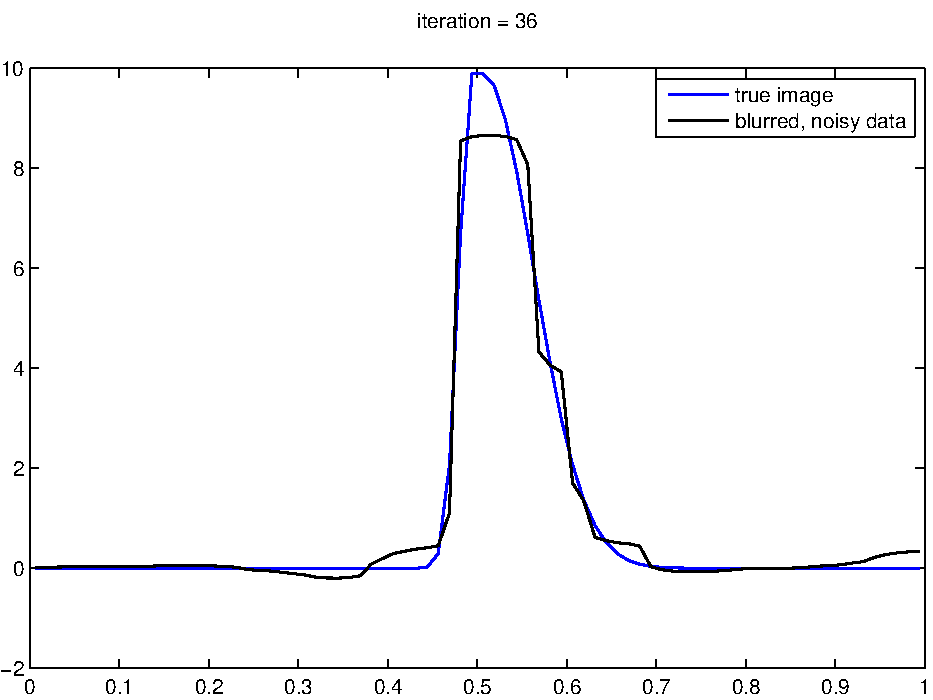
\includegraphics[width=.25\textwidth]{psfrecon_igmrf_02.pdf}
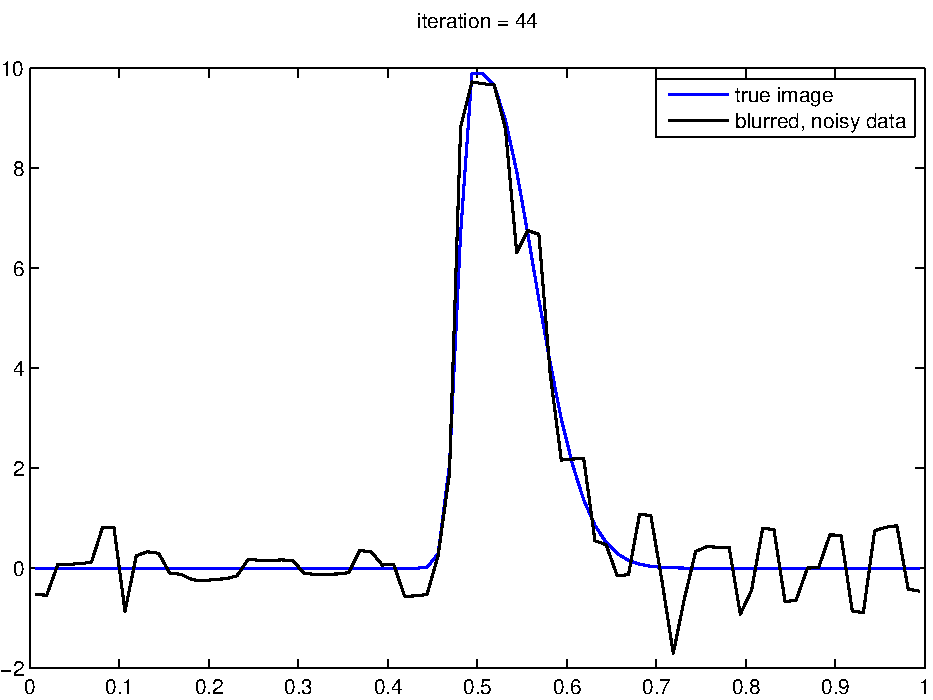
\includegraphics[width=.25\textwidth]{psfrecon_igmrf_03.pdf}
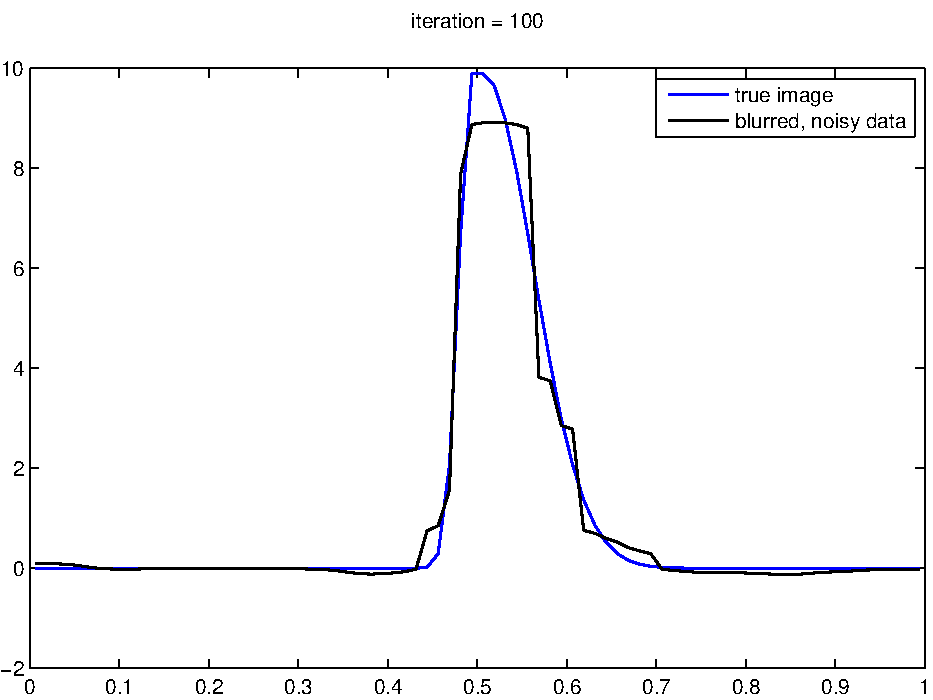
\includegraphics[width=.25\textwidth]{psfrecon_igmrf_04.pdf}

Several MAP estimators with Lagrange priors solved with lagged diffusivity are plotted above. Note the variation between solutions. The stopping criteria for the iterative method was determined by convergence in the estimated sum of squares of the residual $\|\vect{Ax}_\alpha - \vect b\|^2$. The DP was also implemented, but ran only for one iteration most times.  These solutions seem to capture flatness of the tails better, but badly flatten the peak of the PSF.


\end{document}
